\section{Diseño del proyecto, primera iteración}

\subsection{Análisis del problema y de los datos}\label{sec:obtencion}

Considerando que los datos contenidos en los archivos \acrshort{bil} que hemos recibido desde el laboratorio contienen 168 columnas con información de las diferentes longitudes de onda\ \cite{WhatIsHy18:online} y además el nivel de contaminación \gls{don} de cada grano, podemos generar un \gls{dataset} con los datos de cada grano, haciendo la media de cada longitud de onda por cada píxel del mismo grano. Una vez hemos extraído la información de todos los archivos \acrshort{bil} y la hemos guardado en un archivo \acrshort{csv}, podemos entrenar los modelos.

Cabe recalcar que para los modelos de regresión nos hemos guardado el valor de contaminación \gls{don} explícitamente, para los de clasificación si el valor \gls{don} supera los límites de contaminación y hemos preparado un \gls{dataset} aparte con algunos archivos \gls{bil} que contienen granos que no han sido analizados químicamente para el entrenamiento semi-supervisado.

En esta primera iteración nos hemos centrado en intentar encontrar un buen modelo de clasificación y mejorar sus resultados lo máximo posible.

\subsection{Preprocesado de datos}\label{sec:preprocesado}

Ahora que tenemos los datos en un solo archivo \acrshort{csv}, el siguiente paso es preparar los datos. Para ello, hemos realizado el siguiente proceso: 

\begin{enumerate}
    \item Eliminación de columnas
    \item Codificación
    \item Valores atípicos (\textit{outliers})
    \item Balanceo de datos
    \item Separación en datos de entreno y de prueba (\textit{train-test-split})
    \item Preprocesado común, (\textit{pipeline})
    \begin{enumerate}
        \item Separación de datos aplicando la primera derivada 
        \item Aumento de dimensionalidad (\textit{Polynomial Features})
        \item Estandarización  (\textit{Standard Scaler})
        \item Reducción de dimensionalidad (\textit{Principal Component Analysis})
    \end{enumerate}
    
\end{enumerate}


\subsubsection{Eliminación de columnas, codificación y valores atípicos}

Existen datos que nos interesan como medida de seguridad, pero no nos interesa que un modelo entrene con ellos, ya que podría inferir patrones irreales o incluso memorizárselos. En nuestro caso, un ejemplo sería una columna que indicase el número identificador del grano o el archivo del cual se han extraído los datos.

La codificación consiste en transformar columnas con datos categóricos en columnas de datos numéricos, pues los modelos de \acrshort{ml} funcionan mejor con valores numéricos. En nuestro caso, la única columna con valores no numéricos era la columna de la contaminación, que podía tomar los valores \textit{\{B, C\}}, así que lo codificamos manualmente como se muestra a continuación:

{\centering
    \textit{B \longrightarrow{} 0}, \textit{C \longrightarrow{} 1}\par
}

Los valores atípicos u \textit{outliers} son aquellos valores inusuales en los datos que pueden distorsionar nuestros análisis estadísticos. Sin embargo, se debe tener en cuenta que puede haber mucha variación en la naturaleza de nuestro problema. Por ello, se deben diferenciar los \textit{outliers} que se pueden incluir en los datos y los que no. En nuestro caso, los hemos incluido todos, pues al tener cada grano 168 columnas de datos, la mayoría tenía alguna columna que no entraba dentro de lo ``normal'', como por ejemplo en la \textit{figura\ \ref{fig:outliers}}. Por lo que después de probar a quitar todos los granos que alguna de sus columnas fuera un \textit{outlier} (con el \textit{código\ \ref{code:zscore}}), nos quedamos sin datos.

\begin{figure}[!h]
    \centering
    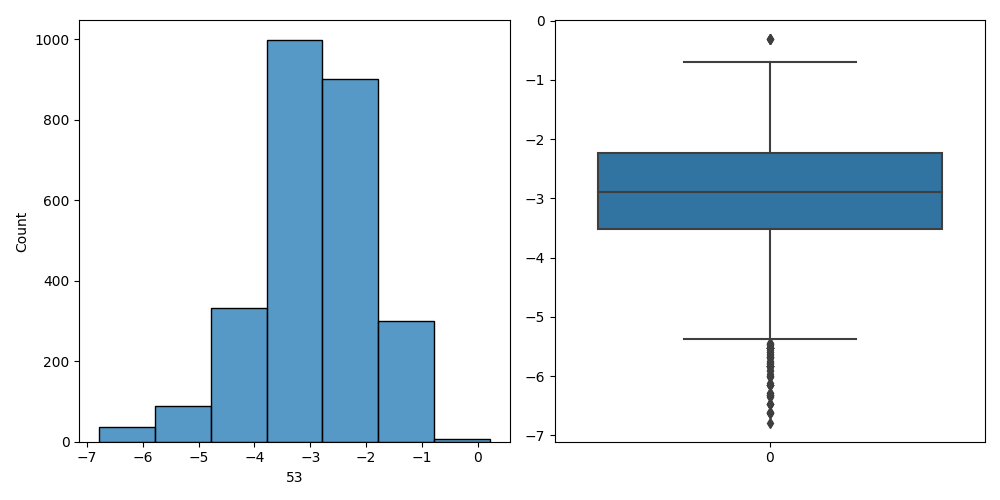
\includegraphics[width=0.7\linewidth]{media/images/col-53-outliers.png}
    \caption{Representación de los \textit{outliers} de la columna 53 en un gráfico de velas, fuente propia, \textit{código\ \ref{code:plot-outliers}}}\ \label{fig:outliers}
\end{figure}


\subsubsection{Balanceo de datos}

Podemos ver en la \textit{figura\ \ref{fig:unbalance}} que los datos no están balanceados, es decir, que la columna que nos interesa `Contaminación' no tiene un número de datos similares en cada clase. En nuestro caso, como en general es más complicado encontrarse un grano contaminado, tenemos más granos sanos.

Al tener las clases desbalanceadas tenemos varias opciones:
\begin{enumerate}
    \item Usar métodos de evaluación que tengan en cuenta el desbalance de las clases.
    \item Balancear el \gls{dataset} utilizando tanto \textit{undersampling} como \textit{oversampling} (explicados en el \textit{apartado\ \ref{sec:i2-balance}}).
\end{enumerate}

Para esta primera iteración, nos es más sencillo utilizar métricas que tengan en cuenta el número de instancias de cada clase a la hora de evaluar los resultados, es decir, que tengan en cuenta el desbalance del \gls{dataset}.

\begin{figure}[!h]
    \centering
    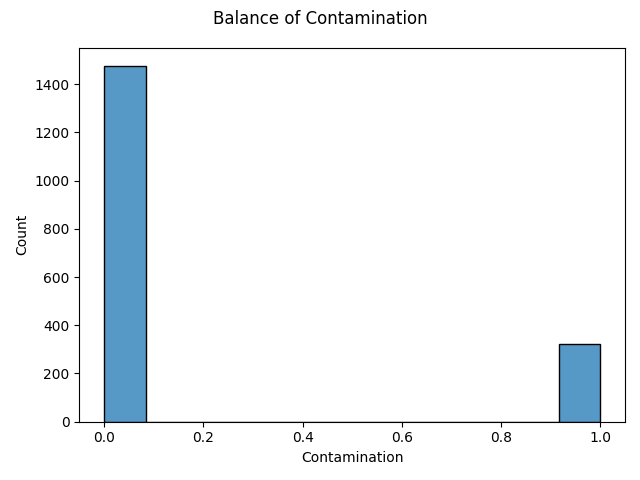
\includegraphics[width=0.7\linewidth]{media/images/unabalance.png}
    \caption{Balanceo de la clase objetivo del \gls{dataset}, fuente propia}\ \label{fig:unbalance}
\end{figure}


\subsubsection{Separación de datos de entreno y de prueba}

En todo el proyecto hemos estado utilizando la librería \href{https://scikit-learn.org/stable/}{sklearn}, esta tiene un submódulo con una función \href{https://scikit-learn.org/stable/modules/generated/sklearn.model_selection.train_test_split.html}{sklearn.model\_selection.train\_test\_split} para separar el \gls{dataset} en entreno y prueba. De todas las opciones, cabe recalcar una que hemos habilitado, pues como en el \gls{dataset} original las etiquetas no están balanceadas y hay muchos más granos sanos que contaminados, es importante que los granos contaminados estén igualmente representados tanto en el conjunto de prueba como en el de entreno. Esto se consigue con la opción \textit{stratify}.


\subsubsection{Preprocesado común}

Después de balancear los datos, debemos transformarlos para que tengan algunas propiedades que suelen ser preferibles a la hora de entrenar ciertos modelos. Es decir, hay modelos que les vendrá mejor tener los datos estandarizados, por ejemplo, y otros que no hará falta o será contraproducente, al final será la prueba y error lo que nos diga qué pasos son preferibles.

Antes de probar diferentes formas de preprocesar los datos, hemos preparado un entorno para entrenar una batería de modelos distintos para ver su efectividad.

Un primer paso, recomendado desde el laboratorio, ya que era lo que utilizaban ellos en su modelo estadístico, es aplicar la primera derivada. El aplicar la derivada permite mínimamente separar los granos contaminados de los que no. Para probarlo, podemos comparar los resultados de entrenar con o sin derivar en la \textit{tabla\ \ref{tab:nopreprocessing-derivative-results}} y, efectivamente, obtenemos resultados algo mejores.

\begin{table}[!h]
    \centering
    \resizebox{\textwidth}{!}{\begin{tabular}{|c|ccccccc|ccccccc|}
        \hline
        & \multicolumn{7}{|c|}{Derivative} & \multicolumn{7}{c|}{No preprocessing} \\ \hline
        Model Name & Train score & Test score & f1score & f0.5score & f2score & ROC/AUC score & Balanced accuracy & Train score & Test score & f1score & f0.5score & f2score & ROC/AUC score & Balanced accuracy \\ \hline
        XGBoost & 82 & 82 & 0 & 0 & 0 & 50 & 50 & 82 & 82 & 0 & 0 & 0 & 50 & 50 \\
        Stochastic Gradient Descent & 18 & 18 & 30.508 & 21.531 & 52.326 & 50 & 50 & 18 & 18 & 30.508 & 21.531 & 52.326 & 50 & 50 \\
        Random Forest & 99.926 & 87.778 & 49.541 & 69.948 & 38.352 & 66.531 & 66.531 & 99.556 & 84.889 & 52.778 & 57.057 & 49.096 & 70.069 & 70.069 \\
        Quadratic Discriminant Analysis & 100 & 82 & 0 & 0 & 0 & 50 & 50 & 100 & 82 & 0 & 0 & 0 & 50 & 50 \\
        Multi-Layer Perceptron & 83.259 & 80.667 & 8.421 & 14.599 & 5.917 & 51.114 & 51.114 & 82 & 82 & 0 & 0 & 0 & 50 & 50 \\
        Linear Discriminant Analysis & 85.333 & 78.222 & 20.968 & 25.692 & 17.711 & 53.96 & 53.96 & 84.889 & 78 & 22.047 & 26.415 & 18.919 & 54.306 & 54.306 \\
        LightGBM & 81.852 & 72 & 47.934 & 40 & 59.794 & 71.846 & 71.846 & 75.778 & 64 & 37.692 & 30.74 & 48.708 & 62.632 & 62.632 \\
        K-Neighbors & 100 & 86.889 & 56.296 & 63.973 & 50.265 & 71.289 & 71.289 & 100 & 91.778 & 74.83 & 79.71 & 70.513 & 82.46 & 82.46 \\
        Hist Gradient Boosting & 78.444 & 70.444 & 44.813 & 37.448 & 55.785 & 68.97 & 68.97 & 72.815 & 63.556 & 33.871 & 28.037 & 42.77 & 58.988 & 58.988 \\
        Extra Trees & 99.63 & 90.444 & 69.504 & 76.324 & 63.802 & 78.756 & 78.756 & 94.667 & 81.111 & 56.853 & 51.376 & 63.636 & 76.438 & 76.438 \\
        Decision Tree & 56.963 & 58.889 & 41.27 & 31.957 & 58.244 & 67.224 & 67.224 & 82 & 82 & 0 & 0 & 0 & 50 & 50 \\ \hline
        & & & & & & 61.79 & 61.79 & & & & & & 59.53572727 & 59.53572727 \\ \hline
        \end{tabular}}
    \caption{Comparación de los resultados de entrenar utilizando la derivada y sin preprocesar. Fuente propia.}\ \label{tab:nopreprocessing-derivative-results}
\end{table}


El siguiente paso que podemos probar es aplicar la transformada, como los resultados habiendo derivado los datos son mejores, transformaremos los datos después de derivarlos. Podríamos probar todas las permutaciones de los diferentes pasos de preprocesado, sin embargo, en esta primera iteración tan solo nos interesa encontrar un resultado decente. Podríamos hacerlo en una segunda o tercera iteración si lo vemos necesario. La transformada consiste en transformar cada columna para que tengan una forma gaussiana\ \cite{sklearnp39:online}. Como estamos utilizando \textit{sklearn}, tenemos una clase que nos aplica la transformada \href{https://scikit-learn.org/stable/modules/generated/sklearn.preprocessing.PowerTransformer.html}{sklearn.preprocessing.PowerTransformer}, por defecto esta clase además te aplica una estandardización de los datos, pero la hemos deshabilitado para aplicarla en otro paso. Podemos ver los resultados de entrenar utilizando la derivada y transformada en la \textit{tabla\ \ref{tab:derivative-transformed-results}}, podemos ver que los resultados son peores, así que continuaremos las pruebas con la derivada.

\begin{table}[!h]
    \centering
    \resizebox{\textwidth}{!}{\begin{tabular}{|c|ccccccc|ccccccc|}
        \hline
            & \multicolumn{7}{|c|}{Transformer and derivative} & \multicolumn{7}{c|}{Derivative} \\ \hline
            Model Name & Train score & Test score & f1score & f0.5score & f2score & ROC/AUC score & Balanced accuracy & Train score & Test score & f1score & f0.5score & f2score & ROC/AUC score & Balanced accuracy \\ \hline
            XGBoost & 82 & 82 & 0 & 0 & 0 & 50 & 50 & 82 & 82 & 0 & 0 & 0 & 50 & 50 \\
            Stochastic Gradient Descent & 18 & 18 & 30.508 & 21.531 & 52.326 & 50 & 50 & 18 & 18 & 30.508 & 21.531 & 52.326 & 50 & 50 \\
            Random Forest & 99.926 & 87.778 & 49.541 & 69.948 & 38.352 & 66.531 & 66.531 & 99.926 & 87.778 & 49.541 & 69.948 & 38.352 & 66.531 & 66.531 \\
            Quadratic Discriminant Analysis & 100 & 83.333 & 19.355 & 34.884 & 13.393 & 55.149 & 55.149 & 100 & 82 & 0 & 0 & 0 & 50 & 50 \\
            Multi-Layer Perceptron & 82 & 82 & 0 & 0 & 0 & 50 & 50 & 83.259 & 80.667 & 8.421 & 14.599 & 5.917 & 51.114 & 51.114 \\
            Linear Discriminant Analysis & 85.185 & 76.667 & 18.605 & 21.978 & 16.129 & 52.529 & 52.529 & 85.333 & 78.222 & 20.968 & 25.692 & 17.711 & 53.96 & 53.96 \\
            LightGBM & 81.852 & 72 & 47.934 & 40 & 59.794 & 71.846 & 71.846 & 81.852 & 72 & 47.934 & 40 & 59.794 & 71.846 & 71.846 \\
            K-Neighbors & 100 & 80.222 & 25.21 & 32.189 & 20.718 & 56.143 & 56.143 & 100 & 86.889 & 56.296 & 63.973 & 50.265 & 71.289 & 71.289 \\
            Hist Gradient Boosting & 78.444 & 70.444 & 44.813 & 37.448 & 55.785 & 68.97 & 68.97 & 78.444 & 70.444 & 44.813 & 37.448 & 55.785 & 68.97 & 68.97 \\
            Extra Trees & 99.63 & 90 & 68.966 & 74.184 & 64.433 & 78.967 & 78.967 & 99.63 & 90.444 & 69.504 & 76.324 & 63.802 & 78.756 & 78.756 \\
            Decision Tree & 56.963 & 58.889 & 41.27 & 31.957 & 58.244 & 67.224 & 67.224 & 56.963 & 58.889 & 41.27 & 31.957 & 58.244 & 67.224 & 67.224 \\ \hline
            & & & & & & 60.669 & 60.669 & & & & & & 61.79 & 61.79 \\ \hline
        \end{tabular}}
    \caption{Comparación de los resultados de entrenar transformando y derivando los datos; frente a solo derivando. Fuente propia.}\ \label{tab:derivative-transformed-results}
\end{table}

A continuación, probaremos la estandarización de los datos como hemos comentado anteriormente. Utilizaremos la clase \href{https://scikit-learn.org/stable/modules/generated/sklearn.preprocessing.StandardScaler.html}{sklearn.preprocessing.StandardScaler}.
La estandardización consiste en el centrado y escalado de los datos. Para ello, columna por columna, restamos la media de los valores (centramos en torno al 0) y 
los dividimos por la varianza (para que la desviación tienda a 1). Tener los datos estandarizados es suele ser un requisito para obtener buenos resultados al entrenar algunos modelos.\ \cite{sklearnp24:online}
Como consecuencia, en la \textit{tabla\ \ref{tab:derivative-standarization-results}} podemos ver que obtenemos mejores resultados.


\begin{table}[!h]
    \resizebox{\textwidth}{!}{\begin{tabular}{|c|ccccccc|ccccccc|}
        \hline
        & \multicolumn{7}{c|}{Derivative + Scaler} & \multicolumn{7}{c|}{Derivative} \\ \hline
        Model Name & Train score & Test score & f1score & f0.5score & f2score & ROC/AUC score & Balanced accuracy & Train score & Test score & f1score & f0.5score & f2score & ROC/AUC score & Balanced accuracy \\ \hline
        XGBoost & 82 & 82 & 0 & 0 & 0 & 50 & 50 & 82 & 82 & 0 & 0 & 0 & 50 & 50 \\
        Stochastic Gradient Descent & 64.815 & 56.444 & 24.615 & 20.075 & 31.809 & 49.834 & 49.834 & 18 & 18 & 30.508 & 21.531 & 52.326 & 50 & 50 \\
        Random Forest & 99.926 & 87.778 & 49.541 & 69.948 & 38.352 & 66.531 & 66.531 & 99.926 & 87.778 & 49.541 & 69.948 & 38.352 & 66.531 & 66.531 \\
        Quadratic Discriminant Analysis & 96.148 & 83.111 & 54.217 & 53.444 & 55.012 & 72.358 & 72.358 & 100 & 82 & 0 & 0 & 0 & 50 & 50 \\
        Multi-Layer Perceptron & 90.815 & 84 & 32.075 & 46.961 & 24.355 & 59.41 & 59.41 & 83.259 & 80.667 & 8.421 & 14.599 & 5.917 & 51.114 & 51.114 \\
        Linear Discriminant Analysis & 85.333 & 78.222 & 20.968 & 25.692 & 17.711 & 53.96 & 53.96 & 85.333 & 78.222 & 20.968 & 25.692 & 17.711 & 53.96 & 53.96 \\
        LightGBM & 82.222 & 72.222 & 48.133 & 40.222 & 59.917 & 71.981 & 71.981 & 81.852 & 72 & 47.934 & 40 & 59.794 & 71.846 & 71.846 \\
        K-Neighbors & 100 & 86.889 & 55.639 & 64.014 & 49.202 & 70.807 & 70.807 & 100 & 86.889 & 56.296 & 63.973 & 50.265 & 71.289 & 71.289 \\
        Hist Gradient Boosting & 78.444 & 70.444 & 44.813 & 37.448 & 55.785 & 68.97 & 68.97 & 78.444 & 70.444 & 44.813 & 37.448 & 55.785 & 68.97 & 68.97 \\
        Extra Trees & 99.63 & 90.444 & 69.504 & 76.324 & 63.802 & 78.756 & 78.756 & 99.63 & 90.444 & 69.504 & 76.324 & 63.802 & 78.756 & 78.756 \\
        Decision Tree & 56.963 & 58.889 & 41.27 & 31.957 & 58.244 & 67.224 & 67.224 & 56.963 & 58.889 & 41.27 & 31.957 & 58.244 & 67.224 & 67.224 \\ \hline
        & & & & & & 64.53009091 & 64.53009091 & & & & & & 61.79 & 61.79 \\ \hline
        \end{tabular}}
    \caption{Comparación de los resultados de entrenar derivando y estandarizando los datos; frente a solo derivando. Fuente propia.}\ \label{tab:derivative-standarization-results}
\end{table}


Además, podemos probar dos últimos pasos que suelen ir juntos. El primero, \href{https://scikit-learn.org/stable/modules/generated/sklearn.preprocessing.PolynomialFeatures.html}{sklearn.preprocessing.PolynomialFeatures}, 
nos permite generar nuevas columnas de datos que consisten en combinar las demás columnas, multiplicándolas entre sí y elevando a un grado específico (segundo grado en nuestro caso). 
De esta forma, teníamos un \gls{dataset} de 168 columnas y obtenemos uno de 14365 columnas. Por ello, debemos aplicar el segundo y último paso para reducir la dimensionalidad
de los datos. Este paso es \href{https://scikit-learn.org/stable/modules/generated/sklearn.decomposition.PCA.html}{sklearn.decomposition.PCA} o \textit{Principal Component Analysis},
reduce la dimensionalidad proyectando los datos a una espacio de menor dimensionalidad. Explicar este proceso más detenidamente se va de nuestro objetivo, pero
aquí podemos leer algo más al respecto sobre \textit{PCA} en \ \cite{Principa62:online}.
Aun añadiendo complejidad de esta forma, podemos ver en la \textit{tabla\ \ref{tab:derivative-standarization-dimensionality-results}} que los resultados son mejores si
nos quedamos en el paso anterior.

\begin{table}[!h]
    \resizebox{\textwidth}{!}{\begin{tabular}{|c|ccccccc|ccccccc|}
        \hline
            & \multicolumn{7}{c|}{Derivative + Scaler + Polynomial Features + PCA} & \multicolumn{7}{c|}{Derivative + Scaler} \\ \hline
            Model Name & Train score & Test score & f1score & f0.5score & f2score & ROC/AUC score & Balanced accuracy & Train score & Test score & f1score & f0.5score & f2score & ROC/AUC score & Balanced accuracy \\ \hline
            XGBoost & 82 & 82 & 0 & 0 & 0 & 50 & 50 & 82 & 82 & 0 & 0 & 0 & 50 & 50 \\
            Stochastic Gradient Descent & 53.333 & 50.444 & 28.754 & 22.299 & 40.468 & 52.439 & 52.439 & 64.815 & 56.444 & 24.615 & 20.075 & 31.809 & 49.834 & 49.834 \\
            Random Forest & 99.926 & 85.778 & 38.462 & 57.803 & 28.818 & 61.939 & 61.939 & 99.926 & 87.778 & 49.541 & 69.948 & 38.352 & 66.531 & 66.531 \\
            Quadratic Discriminant Analysis & 80.889 & 80 & 40 & 42.017 & 38.168 & 63.234 & 63.234 & 96.148 & 83.111 & 54.217 & 53.444 & 55.012 & 72.358 & 72.358 \\
            Multi-Layer Perceptron & 87.778 & 81.778 & 19.608 & 30.303 & 14.493 & 54.682 & 54.682 & 90.815 & 84 & 32.075 & 46.961 & 24.355 & 59.41 & 59.41 \\
            Linear Discriminant Analysis & 82.741 & 81.111 & 6.593 & 12.397 & 4.491 & 50.903 & 50.903 & 85.333 & 78.222 & 20.968 & 25.692 & 17.711 & 53.96 & 53.96 \\
            LightGBM & 77.037 & 68.444 & 38.261 & 32.496 & 46.512 & 62.933 & 62.933 & 82.222 & 72.222 & 48.133 & 40.222 & 59.917 & 71.981 & 71.981 \\
            K-Neighbors & 100 & 83.778 & 42.52 & 50.943 & 36.486 & 64.092 & 64.092 & 100 & 86.889 & 55.639 & 64.014 & 49.202 & 70.807 & 70.807 \\
            Hist Gradient Boosting & 75.63 & 66 & 37.037 & 30.864 & 46.296 & 61.924 & 61.924 & 78.444 & 70.444 & 44.813 & 37.448 & 55.785 & 68.97 & 68.97 \\
            Extra Trees & 96.222 & 82.222 & 51.22 & 50.847 & 51.597 & 70.37 & 70.37 & 99.63 & 90.444 & 69.504 & 76.324 & 63.802 & 78.756 & 78.756 \\
            Decision Tree & 71.852 & 68.889 & 27.835 & 25.328 & 30.892 & 55.014 & 55.014 & 56.963 & 58.889 & 41.27 & 31.957 & 58.244 & 67.224 & 67.224 \\ \hline
            & & & & & & 58.86636364 & 58.86636364 & & & & & & 64.53009091 & 64.53009091 \\ \hline
        \end{tabular}} 
    \caption{Comparación de los resultados de entrenar derivando, estandarizando y ajustando la dimensionalidad de los datos; frente a solo derivando y estandarizando. Fuente propia.}\ \label{tab:derivative-standarization-dimensionality-results}
\end{table}

Por último, es necesario comentar que como tenemos dos aplicaciones (una para entrenar modelos y otra para predecir sobre archivos \gls{bil}),
debemos guardarnos no solo el orden con el que hemos aplicado estos pasos de preprocesado, sino los valores que se han ido ajustando a los datos.
Esto se debe a que cuando uno de estos pasos se aplica sobre los datos de entreno se ajusta a ellos de una u otra forma y realiza un desplazamiento, los datos que debemos guardarnos
son los correspondientes a este desplazamiento. Cada paso almacena sus parámetros, por ejemplo el \textit{StandardScaler} se guarda la media y la varianza de cada columna,
por lo tanto podríamos guardar cada paso con sus parámetros como un archivo binario. Sin embargo, hay una clase que nos ayuda tanto a aplicar el preprocesado como a guardarlo como un solo
archivo `unificado'.\ \textit{Pipeline} nos da la posibilidad de añadir 
una lista de pasos a aplicar secuencialmente sobre un \gls{dataset}. De esta forma aplica los pasos sobre los datos, ajustando los parámetros de cada uno y luego nos permite
guardar el propio \textit{pipeline}, guardando en el tanto el orden de los pasos que lo componen, como los parámetros que representan sus desplazamientos.\ \cite{sklearnp32:online}


\subsection{Entrenamiento de modelos, selección e \textit{hypertuning}}\ \label{sec:entrenamiento}

Ahora que hemos encontrado una combinación de pasos de preprocesado decente, podemos pasar al siguiente paso de selección de los modelos. Aunque hay muchos tipos de modelos 
preparados en la librería, cada uno funciona de una forma distinta. Podríamos investigar cuál funciona mejor con nuestros datos, sin embargo, como el \gls{dataset} que 
tenemos no es muy grande, podemos entrenar todos sin perder mucho tiempo y mirar cuál tiene mejores resultados. Podemos ver en la \textit{tabla\ \ref{tab:best-preprocessing}}
el resultado del mejor preprocesado que hemos encontrado hasta ahora.

\begin{table}[!h]
    \resizebox{\textwidth}{!}{\begin{tabular}{|c|ccccccc|}
        \hline
        & \multicolumn{7}{c|}{Derivative + Scaler} \\ \hline
        Model Name & Train score & Test score & f1score & f0.5score & f2score & ROC/AUC score & Balanced accuracy \\ \hline
        XGBoost & 82 & 82 & 0 & 0 & 0 & 50 & 50 \\
        Stochastic Gradient Descent & 64.815 & 56.444 & 24.615 & 20.075 & 31.809 & 49.834 & 49.834 \\
        Random Forest & 99.926 & 87.778 & 49.541 & 69.948 & 38.352 & 66.531 & 66.531 \\
        Quadratic Discriminant Analysis & 96.148 & 83.111 & 54.217 & 53.444 & 55.012 & 72.358 & 72.358 \\
        Multi-Layer Perceptron & 90.815 & 84 & 32.075 & 46.961 & 24.355 & 59.41 & 59.41 \\
        Linear Discriminant Analysis & 85.333 & 78.222 & 20.968 & 25.692 & 17.711 & 53.96 & 53.96 \\
        LightGBM & 82.222 & 72.222 & 48.133 & 40.222 & 59.917 & 71.981 & 71.981 \\
        K-Neighbors & 100 & 86.889 & 55.639 & 64.014 & 49.202 & 70.807 & 70.807 \\
        Hist Gradient Boosting & 78.444 & 70.444 & 44.813 & 37.448 & 55.785 & 68.97 & 68.97 \\
        Extra Trees & 99.63 & 90.444 & 69.504 & 76.324 & 63.802 & 78.756 & 78.756 \\
        Decision Tree & 56.963 & 58.889 & 41.27 & 31.957 & 58.244 & 67.224 & 67.224 \\ \hline
        & & & & & & 64.53009091 & 64.53009091 \\ \hline
    \end{tabular}}
    \caption{Resultados de entrenar con el mejor preprocesado encontrado. Fuente: propia.}\ \label{tab:best-preprocessing}
\end{table}


Una vez hemos entrenado estos modelos vemos que hay algunos que hacen \textit{overfitting}. 
El \textit{overfitting} ocurre cuando un modelo se ajusta demasiado a los datos con los que ha entrenado y no generaliza bien, es decir que predice mejor los datos con los 
que ha entrenado que datos nuevos.
El modelo con el que lo podemos ver más claramente es el \textit{KNeighbors}, vemos en la \textit{figura\ \ref{fig:lc-knn}} que, para cualquier cantidad de datos con los 
que entrenemos el modelo, siempre predecirá bien con los que ha entrenado y no tanto con los demás. Nuestro objetivo es intentar que ambos valores
no sean tan dispares y que sean lo más altos posibles, para ello haremos \textit{hyperparameter tuning}.

\begin{figure}[!h]
    \centering
    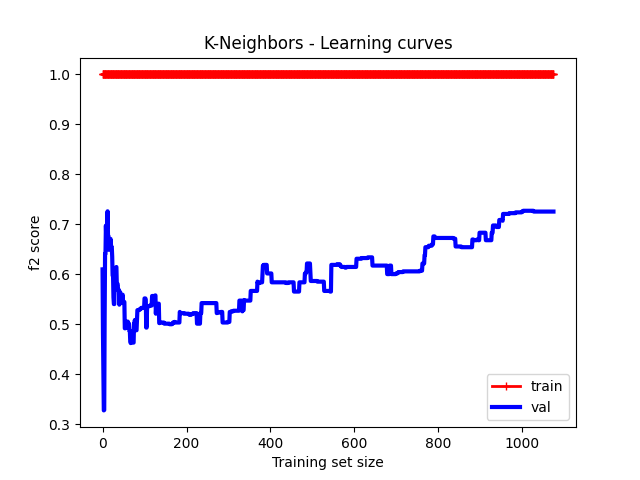
\includegraphics[width=0.7\linewidth]{media/images/learing-curves-knn.png}
    \caption{Gráfico de la curva de aprendizaje del modelo \textit{K-Neighbors} entrenándolo y probándolo sobre los datos de entreno únicamente. Fuente propia}\ \label{fig:lc-knn}
\end{figure}


\subsubsection{Selección de modelos e \textit{hyperparameter tuning}}\ \label{sec:i1-seleccion}

El \textit{hyperparameter tuning} tiene como objetivo encontrar un conjunto de parámetros que maximice el rendimiento del modelo. 
En nuestro caso, como los datos están desbalanceados, podemos utilizar como función de rendimiento el \textit{balanced accuracy}. 
Como cada modelo es distinto, debemos encontrar los parámetros adecuados para cada uno. 
Para ello, para ahorrarnos tiempo podemos utilizar solamente los mejores modelos, como hemos visto en los resultados de la \textit{tabla\ \ref{tab:best-preprocessing}}
hay modelos que tienen mejores resultados que otros.
Así que escogeremos los cuatro con mejor \textit{balanced accuracy}, es decir: \textit{Extra Trees, Quadratic Discriminant Analysis, LightGBM y K-Neighbors}.

Realizaremos el \textit{hyperparameter tuning} en dos pasos, primeramente utilizaremos \textit{Random Search} y después \textit{Grid Search}, ya implementados en \textit{sklearn}.
Ambos métodos utilizan \textit{cross-validation}, una técnica para evitar el \textit{overfitting} que consiste en la división de los datos de entreno en partes iguales.
Una vez dividido en \textit{N} partes, se entrena el modelo sobre todas las partes excepto una, la cual se utiliza para evaluar el modelo entrenado. Entonces, se repite el 
proceso cambiando de partición. De esta forma, haciendo la media obtenemos el resultado de entrenar el modelo repetidas ocasiones con los mismos parámetros, pero con datos 
distintos. Una vez hemos obtenido el mejor de los modelos que hemos entrenado, según la función de rendimiento, probamos el modelo resultante sobre los datos de prueba.
Podemos ver este proceso más gráficamente en la \textit{imagen\ \ref{fig:cross-validation}}.

\begin{figure}[!h]
    \centering
    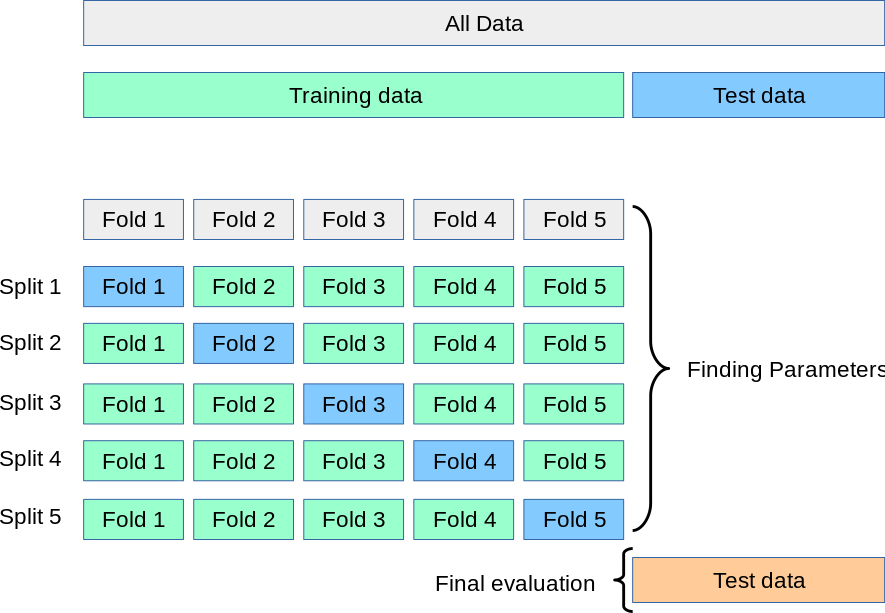
\includegraphics[width=0.7\linewidth]{media/images/cross-validation.png}
    \caption{\textit{Cross-validation} explicado gráficamente. Fuente:\ \cite{31Crossv20:online}}\ \label{fig:cross-validation}
\end{figure}


El \textit{random search} consiste en la búsqueda de estos parámetros habiendo definido un rango de posibilidades. Es decir, para cada parámetro que le queramos
pasar al modelo definiremos un rango de valores que puede tener, entonces el \textit{random search} entrena el modelo repetidas veces con una permutación aleatoria de sus 
parámetros y se guarda los resultados. Podemos ver un ejemplo en el \textit{código\ \ref{code:random-search-example}}.
Podemos ir probando diferentes parámetros y rangos hasta que estemos satisfechos con el resultado.


Una vez estemos contentos con los resultados, los refinaremos utilizando \textit{grid search}. A diferencia del \textit{random search}, el \textit{grid search} prueba todas
las posibles combinaciones que le pasemos como parámetro y, consecuentemente, es mucho más lento. Por ello, utilizaremos el \textit{grid search} con los mejores parámetros que
encontremos del paso anterior, los cuales son potencialmente los mejores. Una vez definido un rango de parámetros para los modelos seleccionados, obtenemos los resultados
de la \textit{tabla\ \ref{tab:hyperparameter-tuning-results}}. Podemos ver que hemos obtenido, en general, peores resultados (salvo con \textit{K-Neighbors}), por lo tanto
deberíamos ajustar el rango de parámetros que les pasamos a los modelos y volver a entrenarlos hasta que estemos satisfechos con el resultado. En nuestro caso no lo haremos
y pasaremos a la segunda iteración del proyecto para probar nuevas cosas en pasos anteriores.

\begin{table}
    \resizebox{\textwidth}{!}{\begin{tabular}{|c|ccccccc|}
            \hline
            Model name & Train score & Accuracy & f1 score & f0.5 score & f2 score & ROC/AUC score & Balanced accuracy \\ \hline
            RS - knn & 100 & 90.274 & 85.897 & 87.927 & 83.96 & 90.274 & 90.274 \\
            GS - knn & 100 & 90.274 & 85.897 & 87.927 & 83.96 & 90.274 & 90.274 \\
            RS - qda & 97.491 & 72.358 & 54.217 & 53.444 & 55.012 & 72.358 & 72.358 \\
            GS - qda & 97.491 & 72.358 & 54.217 & 53.444 & 55.012 & 72.358 & 72.358 \\
            RS - lgbm & 86.013 & 71.018 & 47.257 & 39.716 & 58.333 & 71.018 & 71.018 \\
            GS - et & 82.957 & 66.17 & 43.077 & 39.106 & 47.945 & 66.17 & 66.17 \\
            GS - lgbm & 84.628 & 70.626 & 46.215 & 38.108 & 58.704 & 70.626 & 70.626 \\
            RS - et & 69.492 & 65.854 & 40.909 & 33.21 & 53.254 & 65.854 & 65.854 \\\hline
            \end{tabular}
    }
    \caption{Resultados del primer entrenamiento con hyperparameter tuning. Fuente propia.}\ \label{tab:hyperparameter-tuning-results}
\end{table}

